\documentclass{article}
    \author{杨铭\\5130379022}
    \title{Homework - SIFT}
\usepackage{ctex}
\usepackage{graphicx}
\begin{document}
    \maketitle
    \section{简述}
        \paragraph{}主要代码在SIFT.py中,使用python编写,调用了random库在绘制匹配点对及其连线时生成随机颜色,以及opencv的python
    接口实现对各种格式图像的读取和写入
    \section{输入格式}
        \paragraph{}使用opencv的cv2.imread函数读取图片,支持.bmp,.jpg.png等格式
    \section{实现方式}
        \paragraph{调用opencv2.4的SIFT及其算法完成对两幅图的特征提取和匹配}
            \subparagraph{版本说明}由于之前使用的opencv3.0默认没有SIFT模块,我将其版本降为了2.4.10,并且自己实现了相应的drawMatchesKnn方法
        \section{结果}
        \paragraph{分析}最开始在调用SIFT算子时,应该注意控制特征点数和层数,否则在应对不同情况时不能达到很好的效果
        \paragraph{}另外,opencv对python的支持有点坑,各种版本兼容问题
        \paragraph{结果图}下面是一张动漫图片和两张自己拍摄的校园照片的处理结果
        \begin{figure}[htbp]
                \begin{minipage}[t]{0.5\linewidth}
                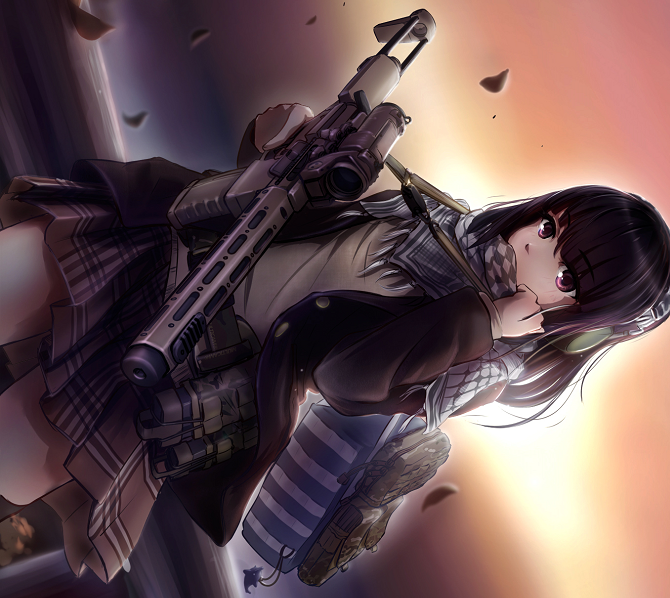
\includegraphics[width=4cm]{test1.png}
                \caption{匹配图}\label{1-a}
                \end{minipage}
                \begin{minipage}[t]{0.5\linewidth}
                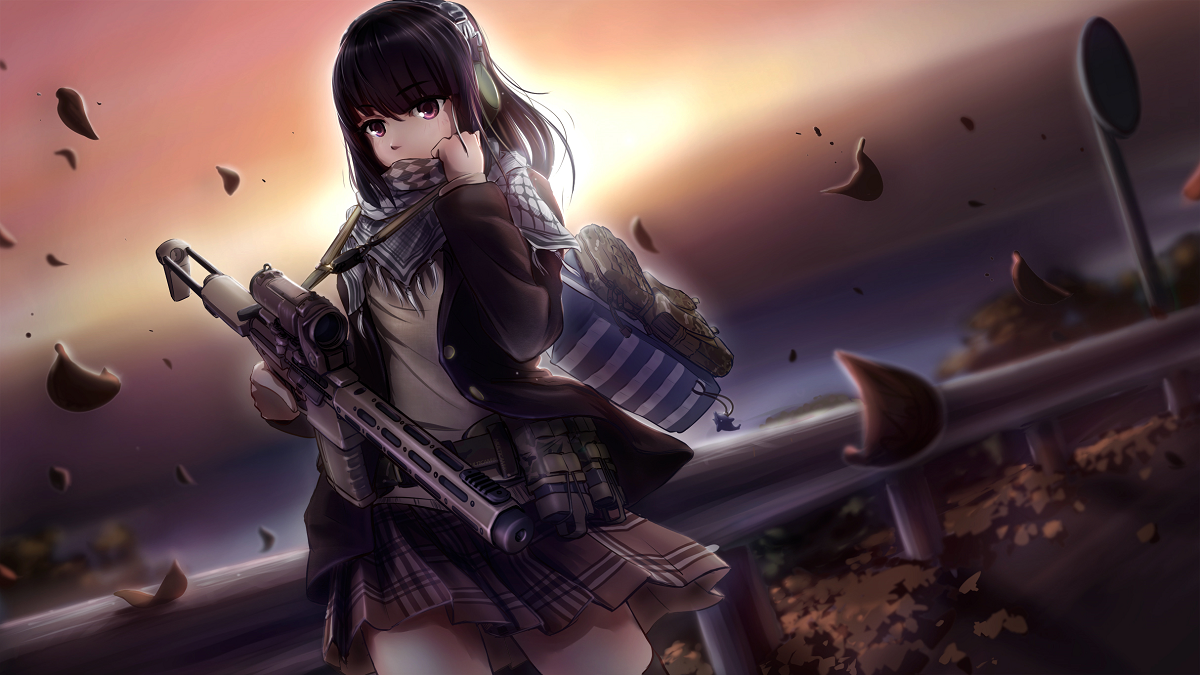
\includegraphics[width=8cm]{test2.png}
                \caption{原图}\label{1-b}
                \end{minipage}
                \begin{minipage}[t]{1\linewidth}\centering
                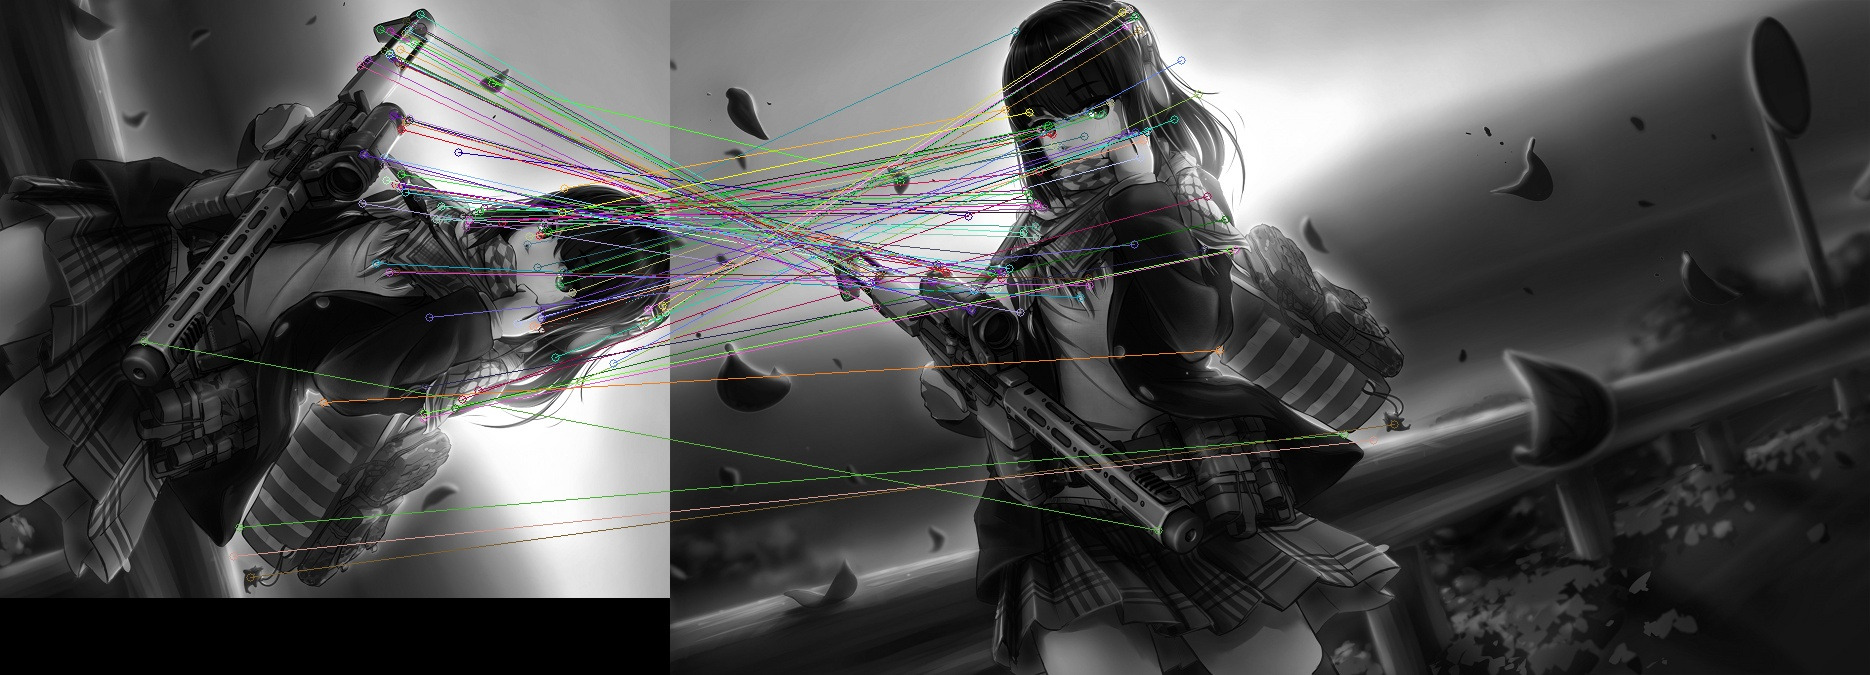
\includegraphics[width=12cm]{sift_matches.jpg}
                \caption{SIFT算法匹配:nfeatures=150,nOctaveLayers=6}\label{1-c}
                \end{minipage}
        \end{figure}
        \begin{figure}[htbp]
                \begin{minipage}[t]{0.5\linewidth}\centering
                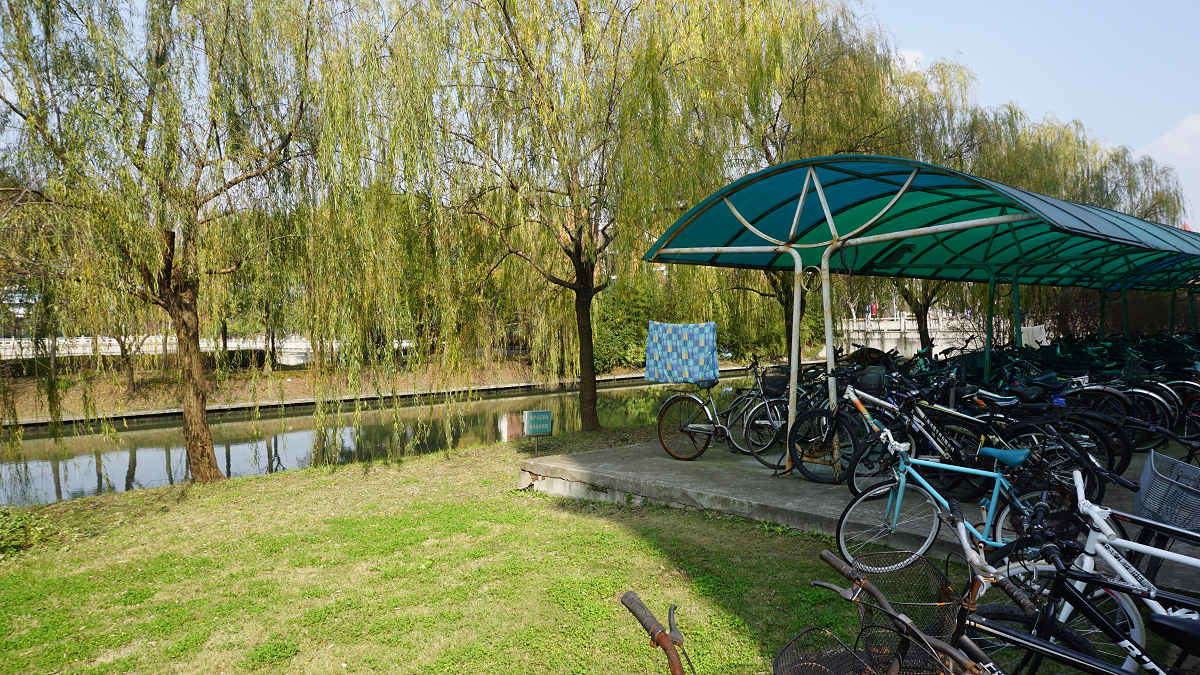
\includegraphics[width=6cm]{Pic1-1.png}
                \caption{匹配图}\label{2-a}
                \end{minipage}
                \begin{minipage}[t]{0.5\linewidth}\centering
                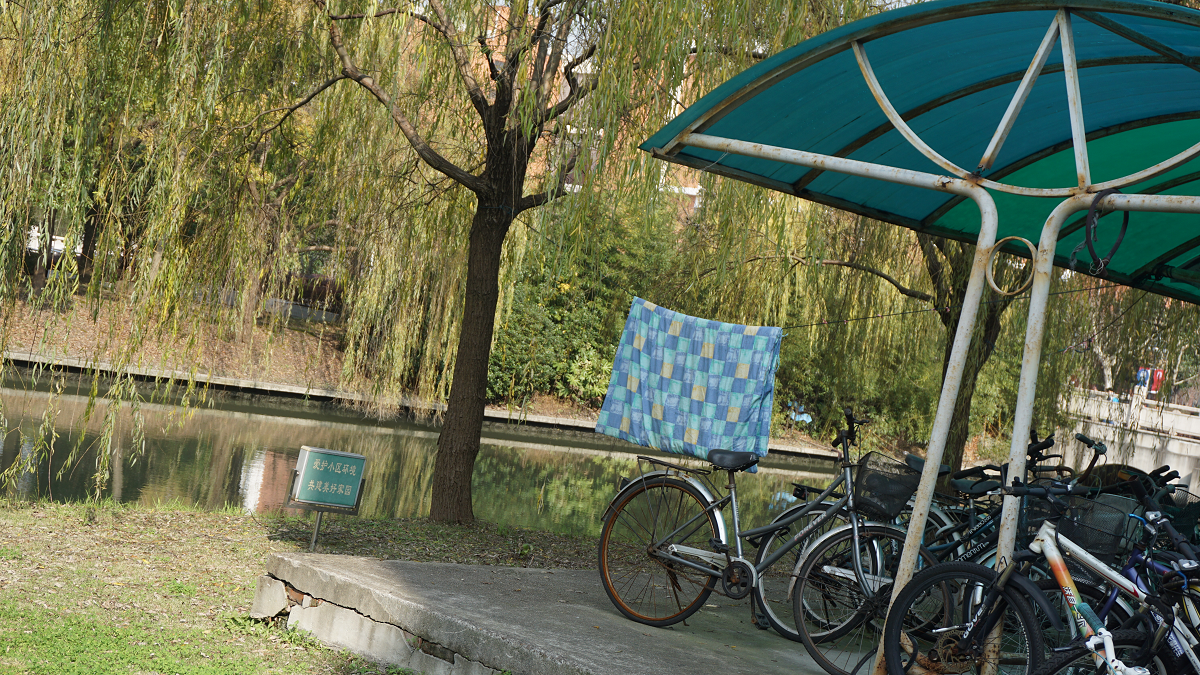
\includegraphics[width=6cm]{Pic1-2.png}
                \caption{原图}\label{2-b}
                \end{minipage}
                \begin{minipage}[t]{1\linewidth}\centering
                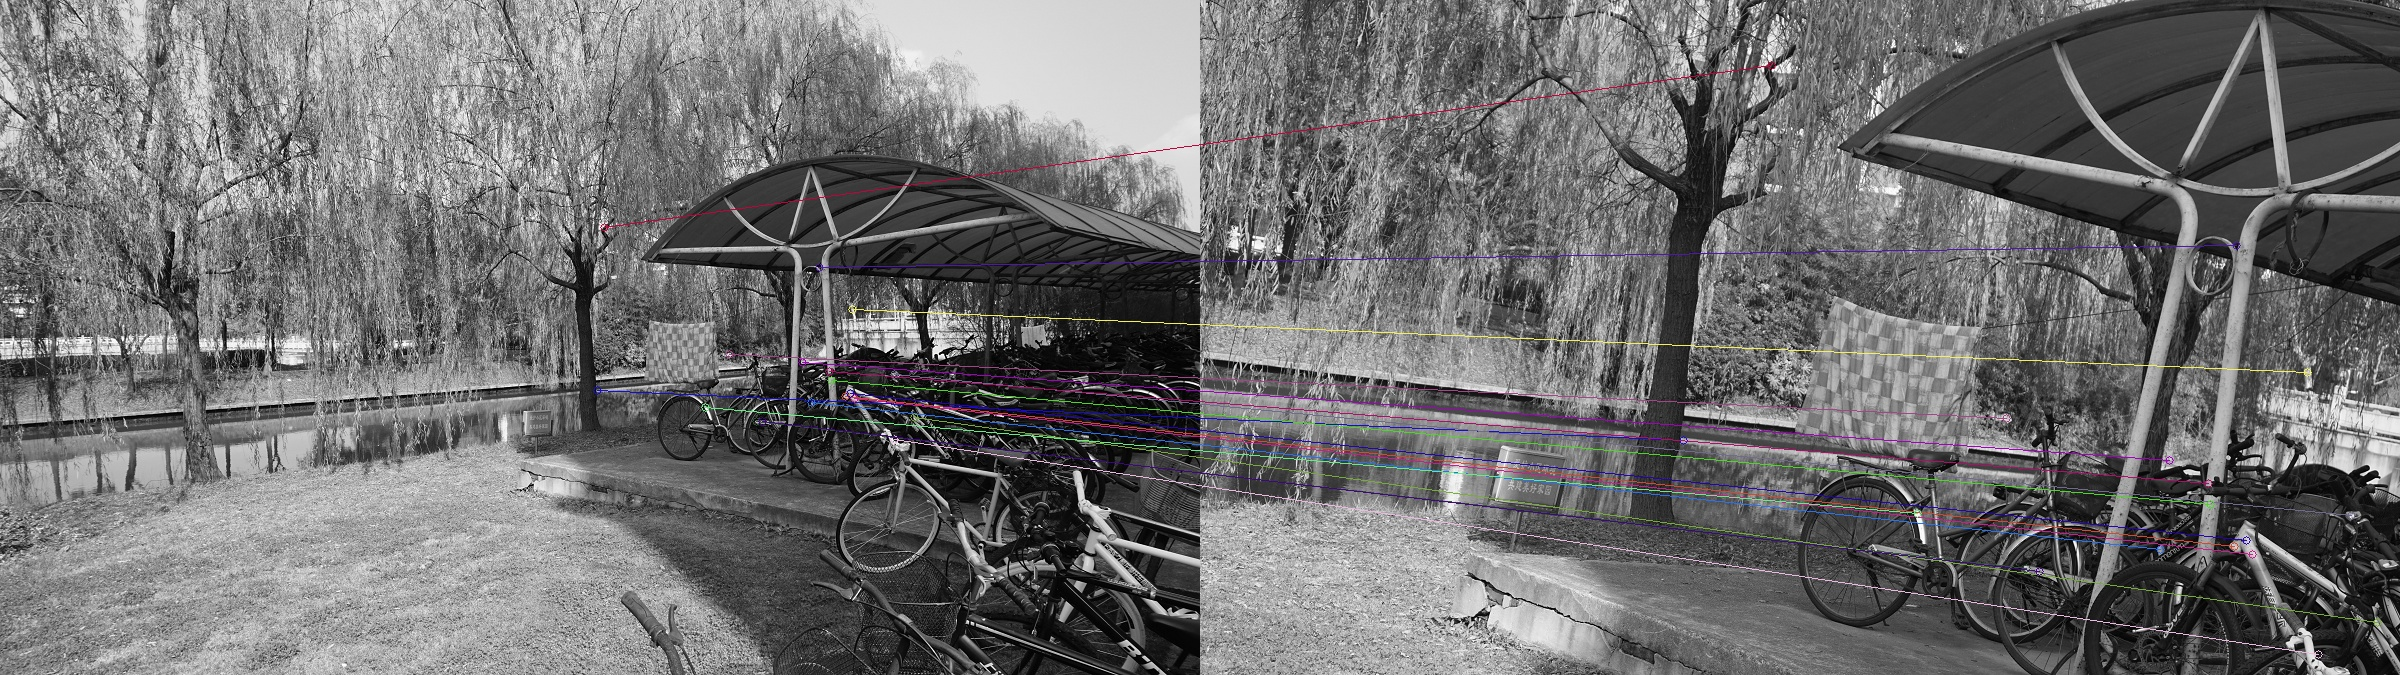
\includegraphics[width=12cm]{sift_matches_Pic1.jpg}
                \caption{SIFT算法匹配:nfeatures=500,nOctaveLayers=5}\label{2-c}
                \end{minipage}
        \end{figure}
        \begin{figure}[htbp]
                \begin{minipage}[t]{0.5\linewidth}\centering
                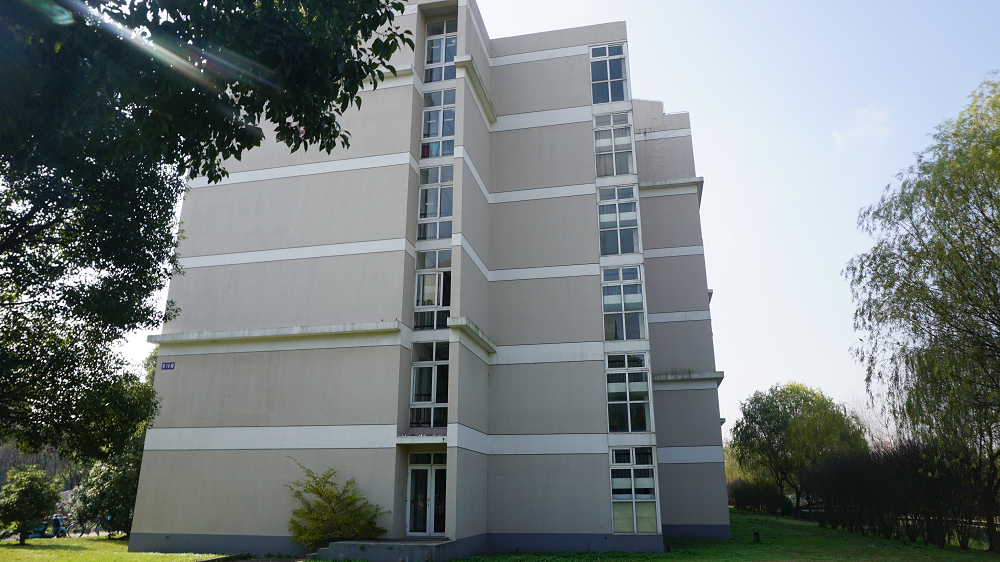
\includegraphics[width=6cm]{Pic2-1.png}
                \caption{匹配图}\label{3-a}
                \end{minipage}
                \begin{minipage}[t]{0.5\linewidth}\centering
                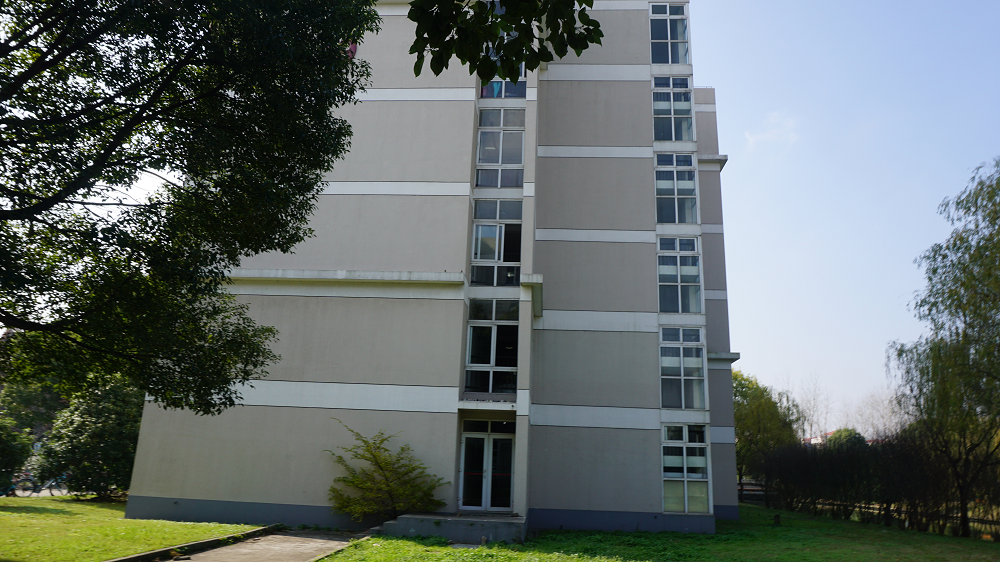
\includegraphics[width=6cm]{Pic2-2.png}
                \caption{原图}\label{3-b}
                \end{minipage}
                \begin{minipage}[t]{1\linewidth}\centering
                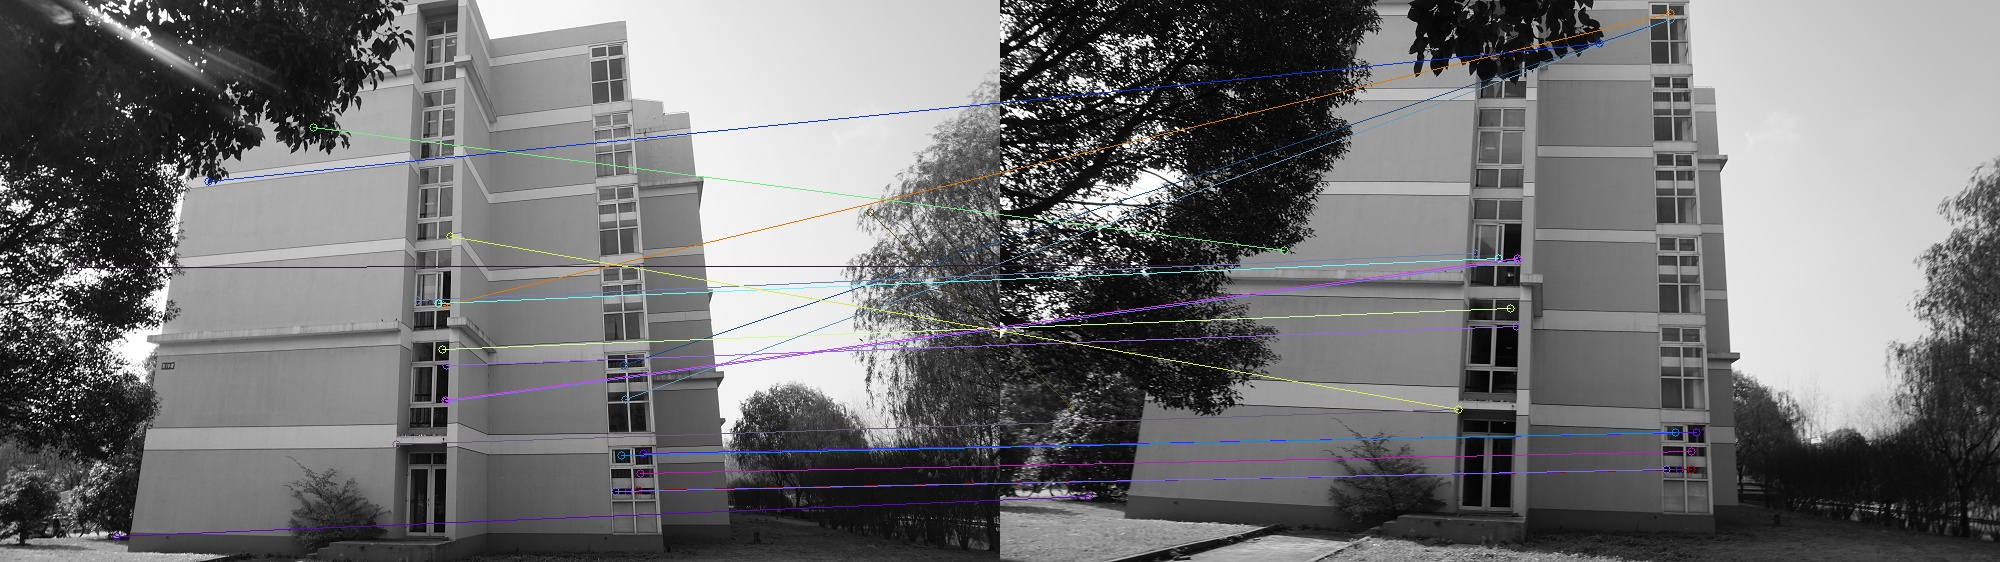
\includegraphics[width=12cm]{sift_matches_Pic2.jpg}
                \caption{SIFT算法匹配:nfeatures=1000,nOctaveLayers=6}\label{3-c}
                \end{minipage}
        \end{figure}
\end{document}
